\documentclass[svgnames, 12pt]{beamer}

\usepackage[utf8]{inputenc}
\usepackage[english]{babel}
\usepackage[L7x]{fontenc}
\usepackage{lmodern}
\usepackage{amsmath}
\usepackage{amssymb}
\usepackage{xcolor}
\usepackage{subfig}
\usepackage{graphicx}
\usepackage{lipsum}
\usepackage{hyperref}

\definecolor{mifcolor}{RGB}{0, 71, 127}
\definecolor{dimgr}{RGB}{105, 105, 105}
\definecolor{sky}{RGB}{0, 191, 255}
\setbeamercolor{alerted text}{fg=red,bg=sky}
\newcommand{\boxalert}[1]{{%
	\usebeamercolor{alerted text}\colorbox{bg}{\alert{#1}}%
}}

\mode<presentation>{
\usetheme{Madrid}
\usecolortheme[named=mifcolor]{structure}
\setbeamertemplate{footline}
{%
	\leavevmode%
	\hbox{ \begin{beamercolorbox}[wd=.3\paperwidth,ht=2.5ex,dp=1.125ex,leftskip=.3cm
			plus1fill,rightskip=.3cm]{author in head/foot}%
			\usebeamerfont{author in head/foot}\insertshortauthor \hfill 
		\end{beamercolorbox}%
		\begin{beamercolorbox}[wd=.2\paperwidth,ht=2.5ex,dp=1.125ex,leftskip=.3cm,
			rightskip=.3cm plus1fil]{institute in head/foot}%
			\usebeamerfont{institute in head/foot}\insertshortinstitute
		\end{beamercolorbox}%
		\begin{beamercolorbox}[wd=.2\paperwidth,ht=2.5ex,dp=1.125ex,leftskip=.3cm,
			rightskip=.3cm plus1fil]{date in head/foot}%
			\usebeamerfont{date in head/foot}\insertshortdate
		\end{beamercolorbox}%
		\begin{beamercolorbox}[wd=.3\paperwidth,ht=2.5ex,dp=1.125ex,leftskip=.3cm,
			rightskip=.3cm plus1fil]{title in head/foot}%
			\usebeamerfont{title in head/foot}\insertshorttitle\hfill p.
			\insertframenumber\enspace of \inserttotalframenumber\enspace 
	\end{beamercolorbox} }%
	\vskip0pt%
}
}

\title[FDA of Weather Data]{Functional Data Analysis of Weather Data}%
\author[A. J. Smoliakov]{Aleksandr Jan Smoliakov\inst{1}}
\institute[VU MIF]{\inst{1} Vilnius University, Faculty of Mathematics and Informatics}
\date{2025--04--29}

\begin{document}

\begin{frame}

\includegraphics[scale=0.15]{MIF Garamond-logo.png} 
\hfill

\includegraphics[scale=0.15]{Logo_spalvotas.eps}

\titlepage
\end{frame}

\begin{frame}{Table of Contents}
\tableofcontents
\end{frame}

\section{Data Source}

\begin{frame}{Data Source}
			\begin{itemize}
		\item \textbf{Historical Weather Data in India}
		\begin{itemize}
			\item Hourly observations (2006--2019)
			\item 8 major Indian cities
			\item Over 20 meteorological variables (focus on Temperature)
		\end{itemize}
			\end{itemize}
\end{frame}

\section{Research Questions}

\begin{frame}{Research Questions}
	\begin{itemize}
		\item \textbf{Main goal:} Explore seasonal patterns in temperature data.
		\item \textbf{Questions:}
		\begin{itemize}
			\item How do daily temperature curves differ by season?
			\item Can yearly and intra-day temperature patterns be identified?
			\item Are there consistent patterns in the derivatives of the curves?
		\end{itemize}
	\end{itemize}
\end{frame}

\section{Temperature Curves}

\begin{frame}{Unsmoothed Temperature Curves}
	\begin{itemize}
		\item Daily temperature profiles from Mumbai in 2011.
		\item Lines colored by season (winter, spring, summer, fall).
		\item "Stepwise" appearance due to hourly observations.
	\end{itemize}
	\begin{center}
		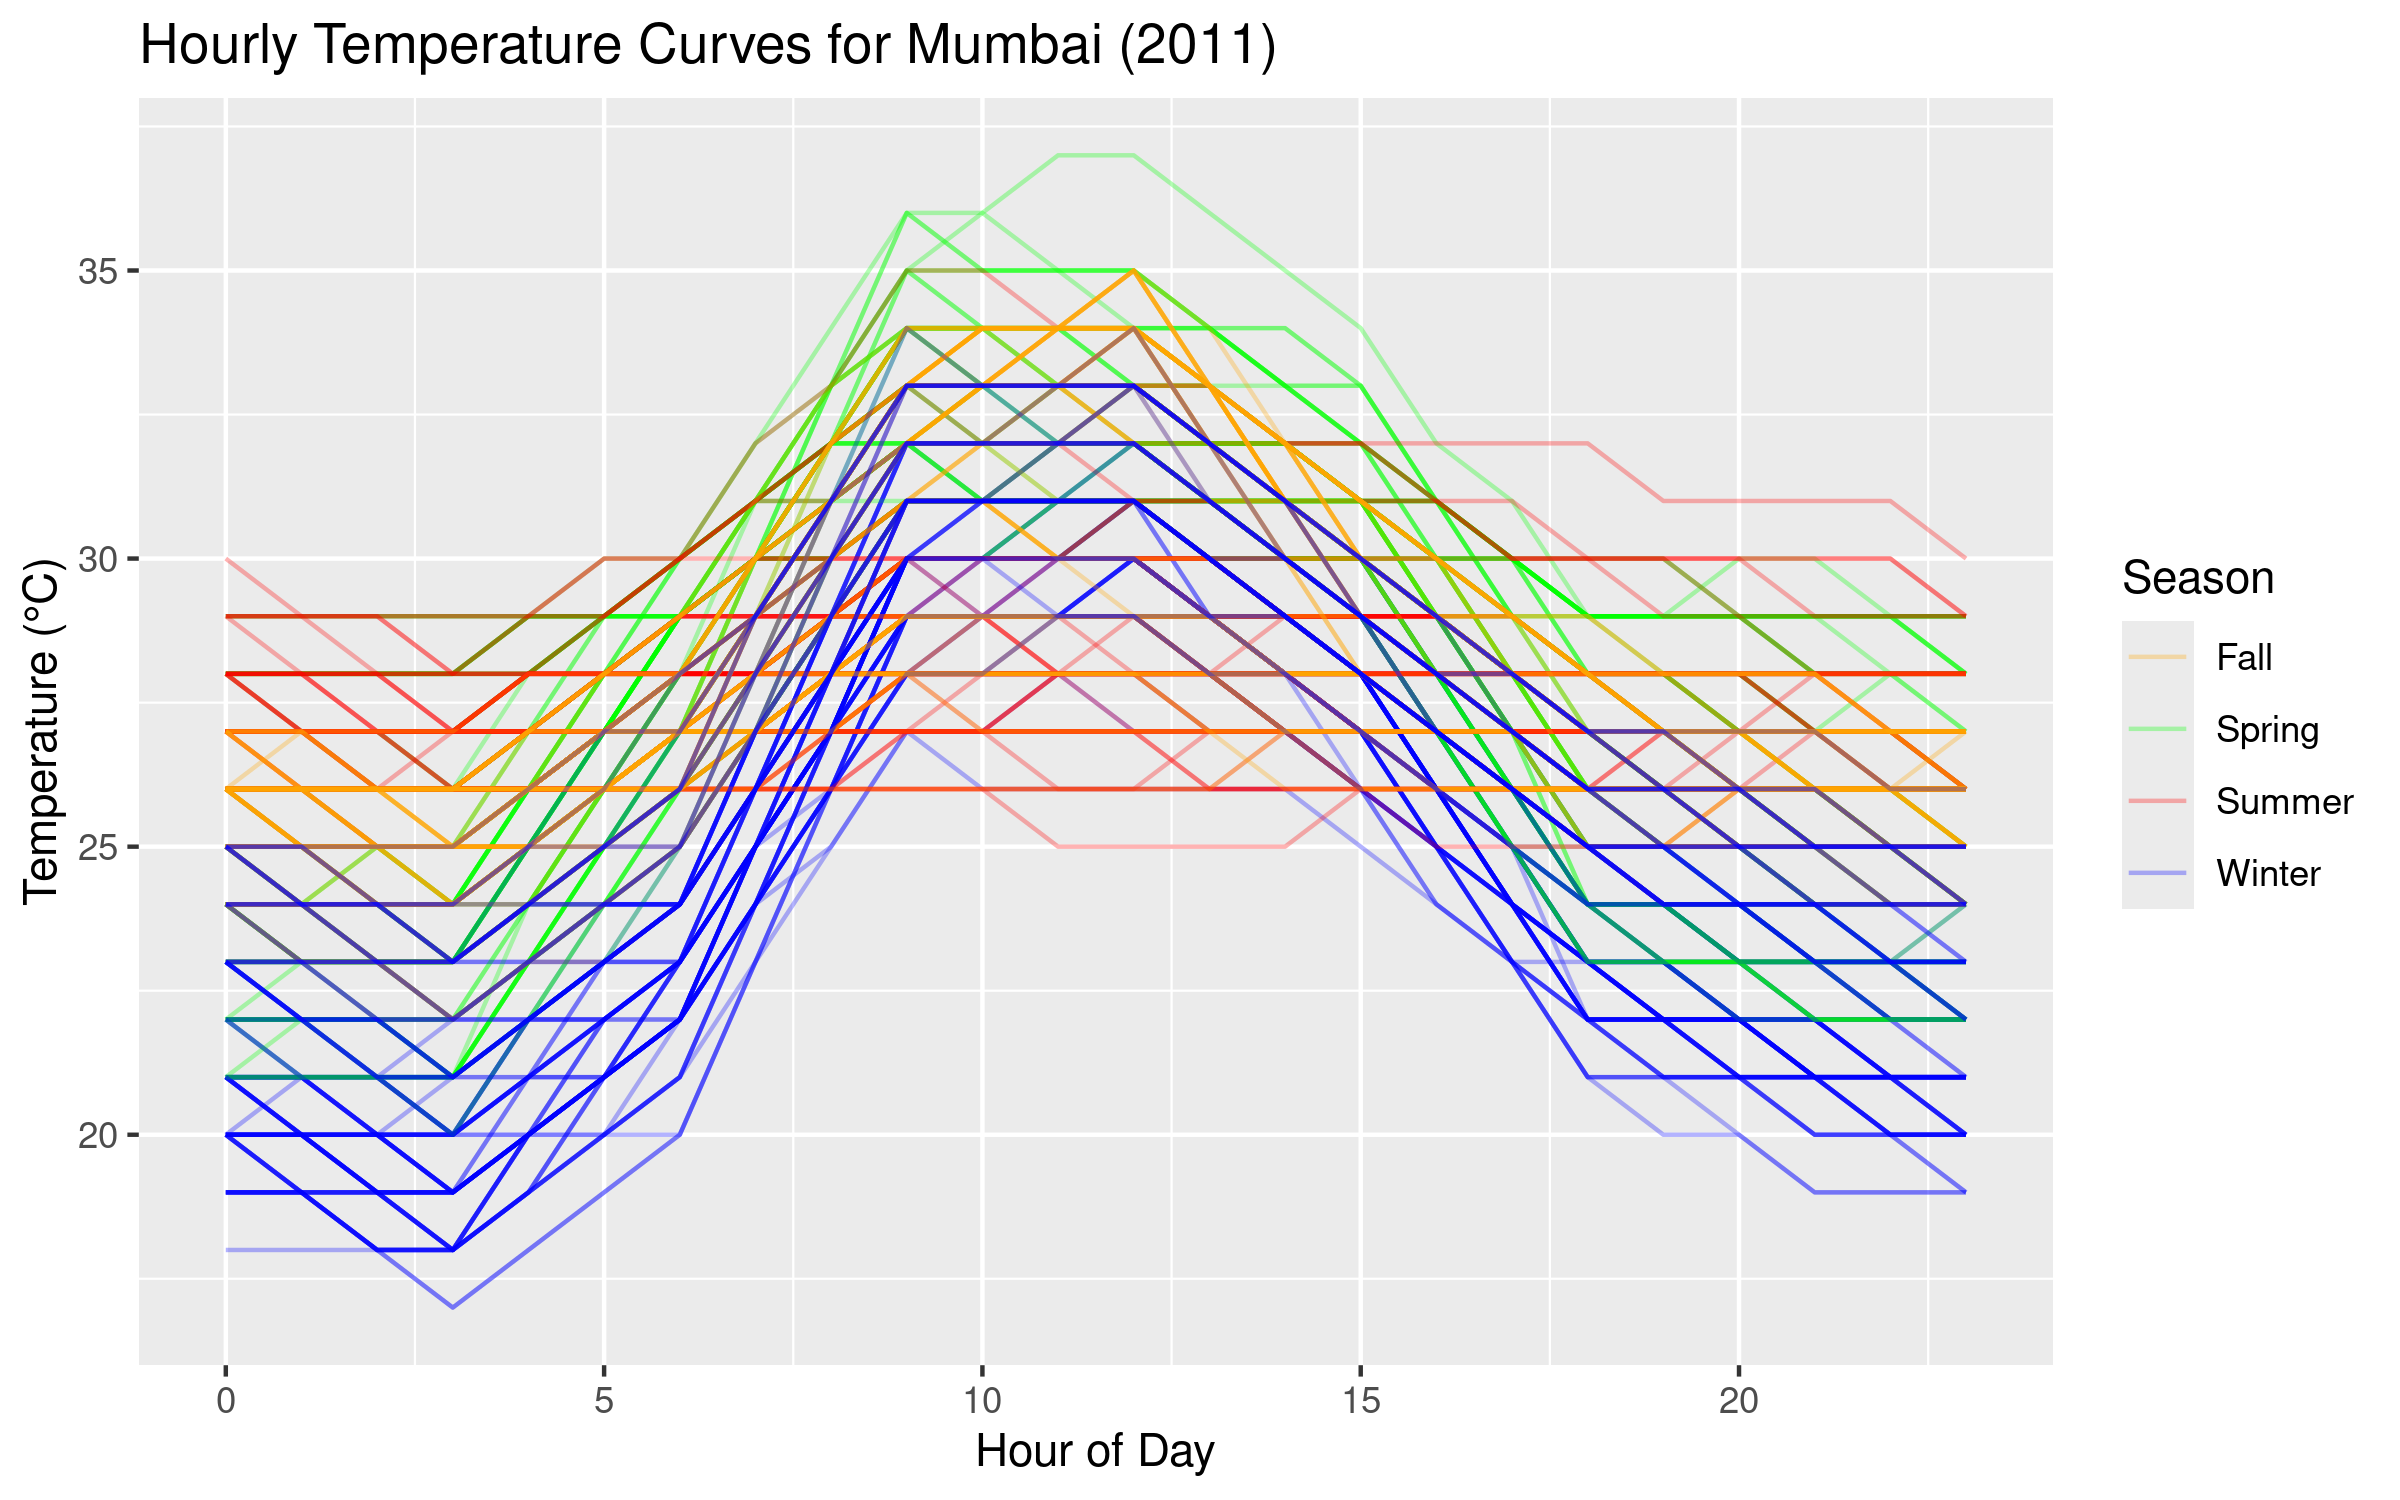
\includegraphics[width=0.8\linewidth]{../notebooks/assets/unsmoothed_temp_curves_mumbai.png}
	\end{center}
\end{frame}

\section{Basis \& Smoothing}
\begin{frame}{Lambda Selection via GCV}
	\begin{itemize}
		\item Bivariate smoothing: B-splines in \emph{day} (nbasis=12), Fourier in \emph{hour} (harmonics=5)
		\item Search $\lambda\in[10^{-4},10^1]$ to minimize GCV
		\item Optimal $\lambda_{opt}$ indicated by dashed line (selected $\lambda=\epsilon=10^{-7}$)
	\end{itemize}
	\vfill
	\begin{center}
		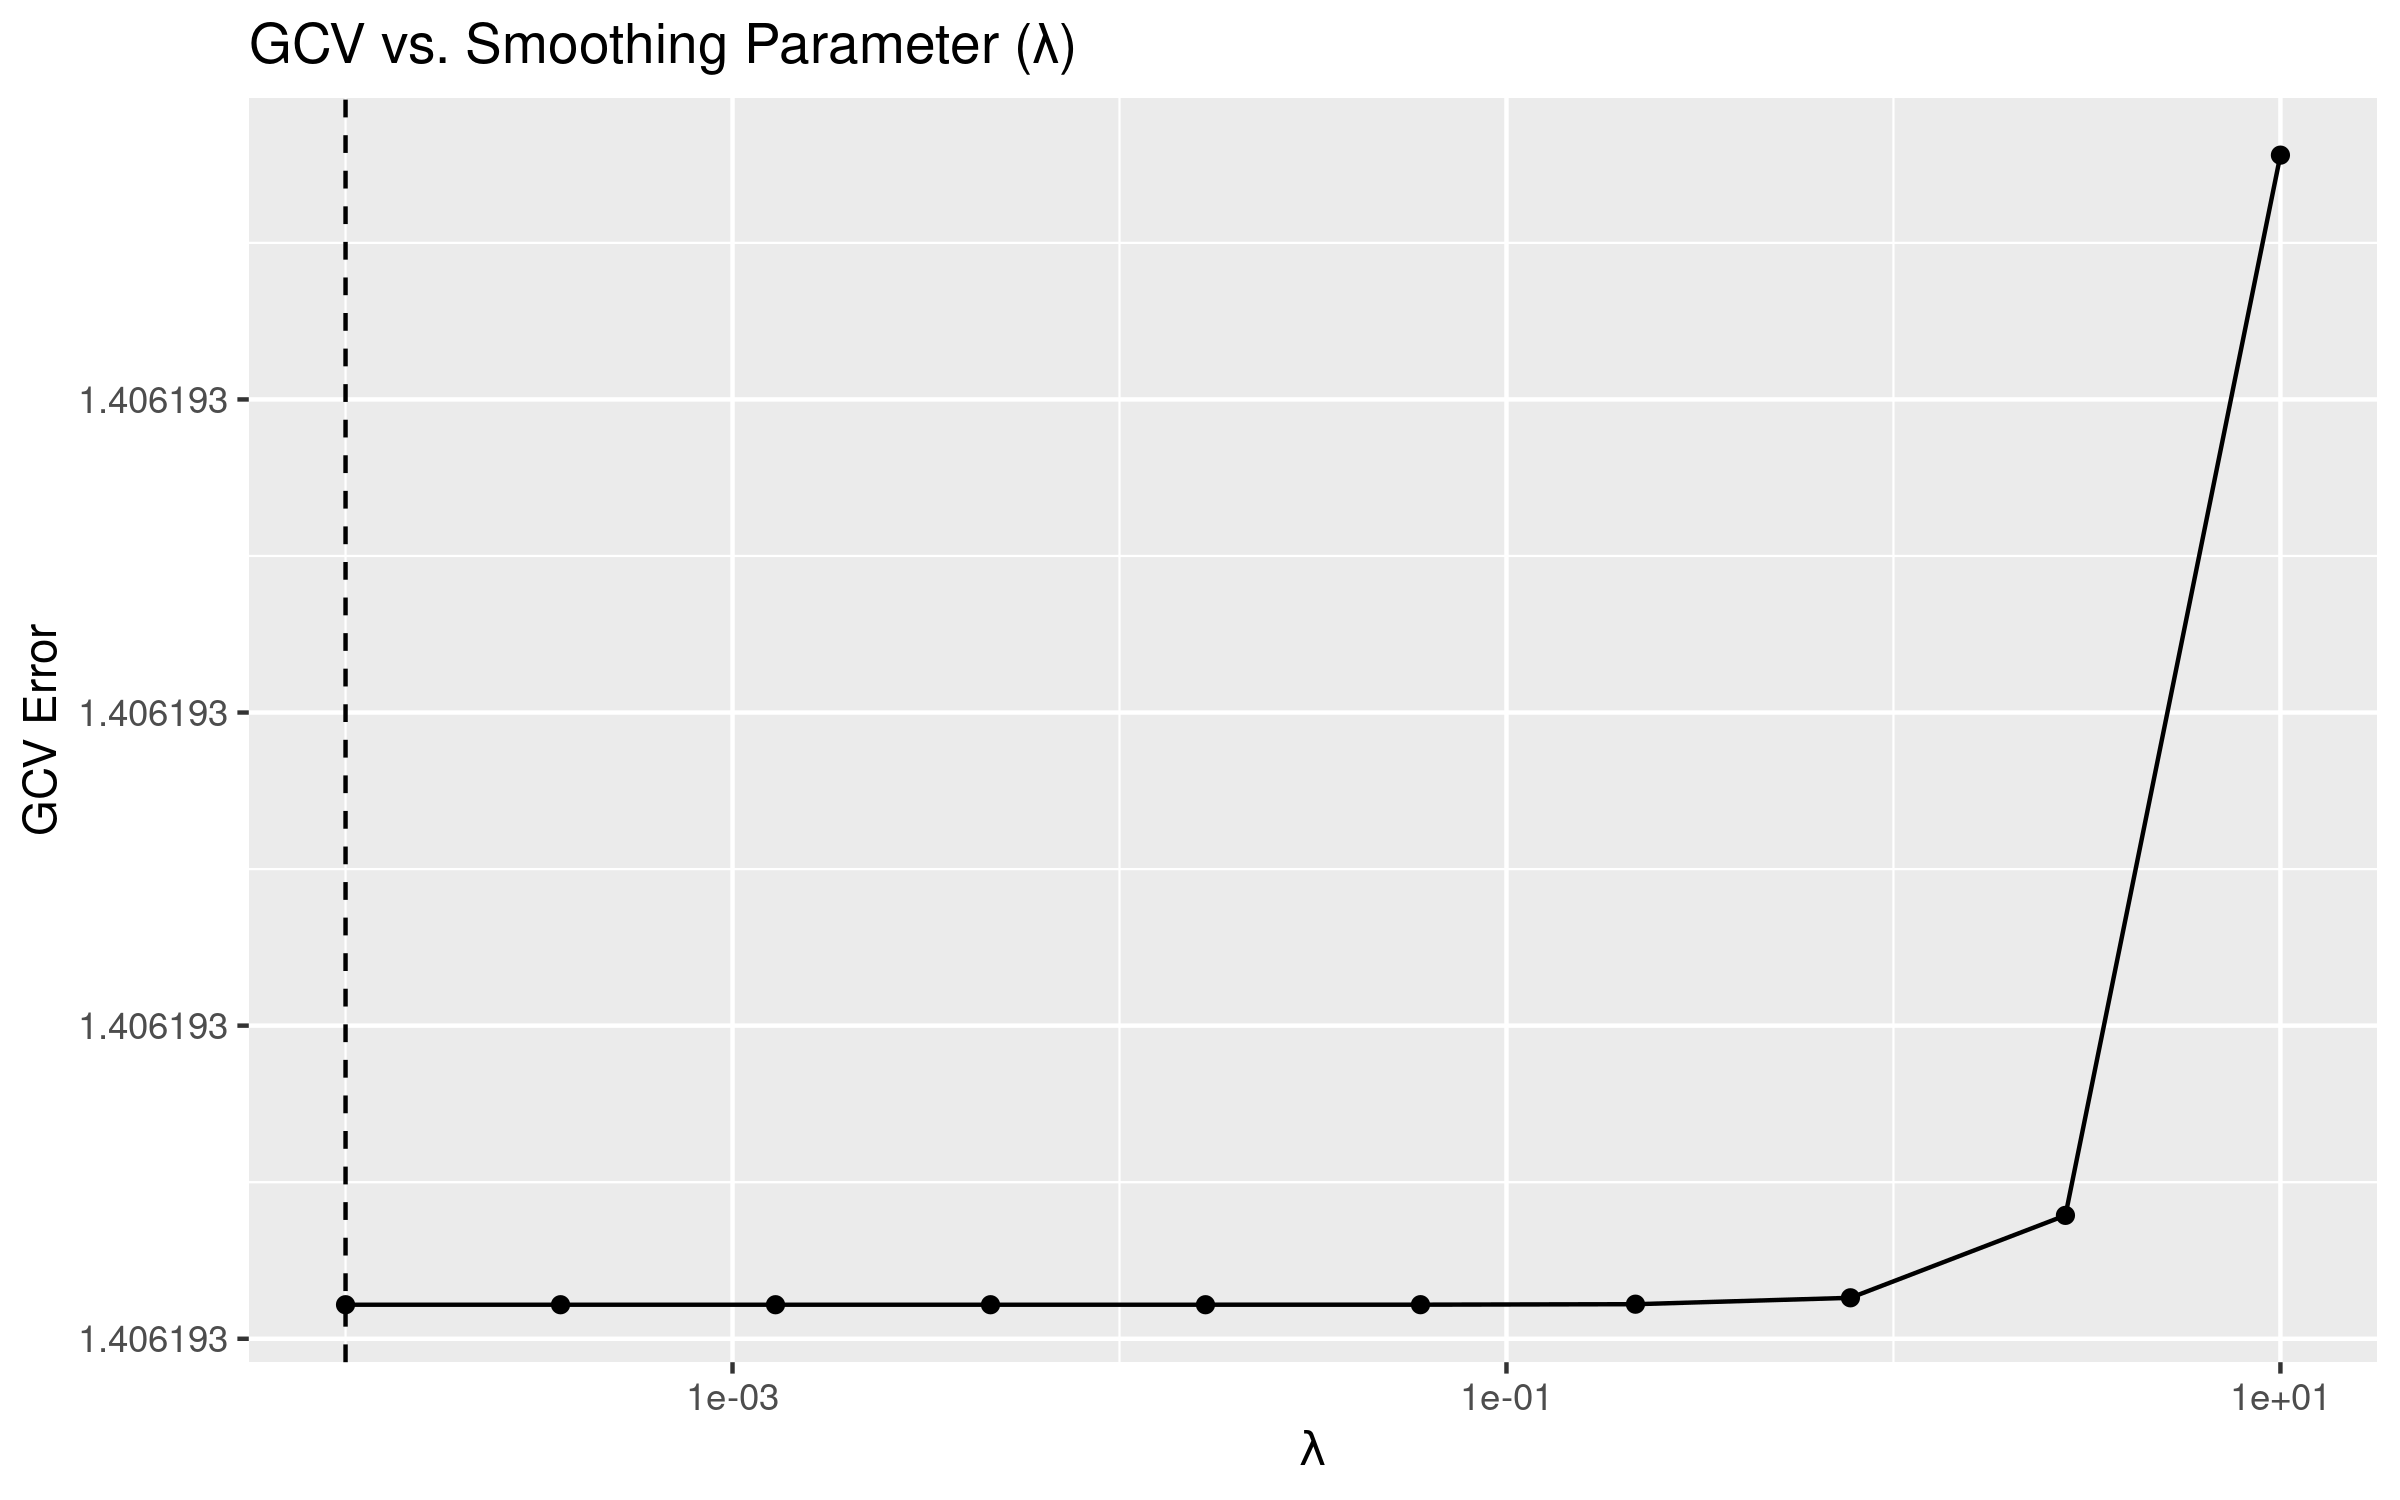
\includegraphics[width=0.7\linewidth]{../notebooks/assets/gcv_vs_lambda.png}
	\end{center}
\end{frame}

\begin{frame}{Smoothed Temperature Curves}
	\begin{itemize}
		\item Applied bivariate smoothing with $\lambda_{opt}$
		\item Reveals underlying daily patterns by season
	\end{itemize}
	\begin{center}
		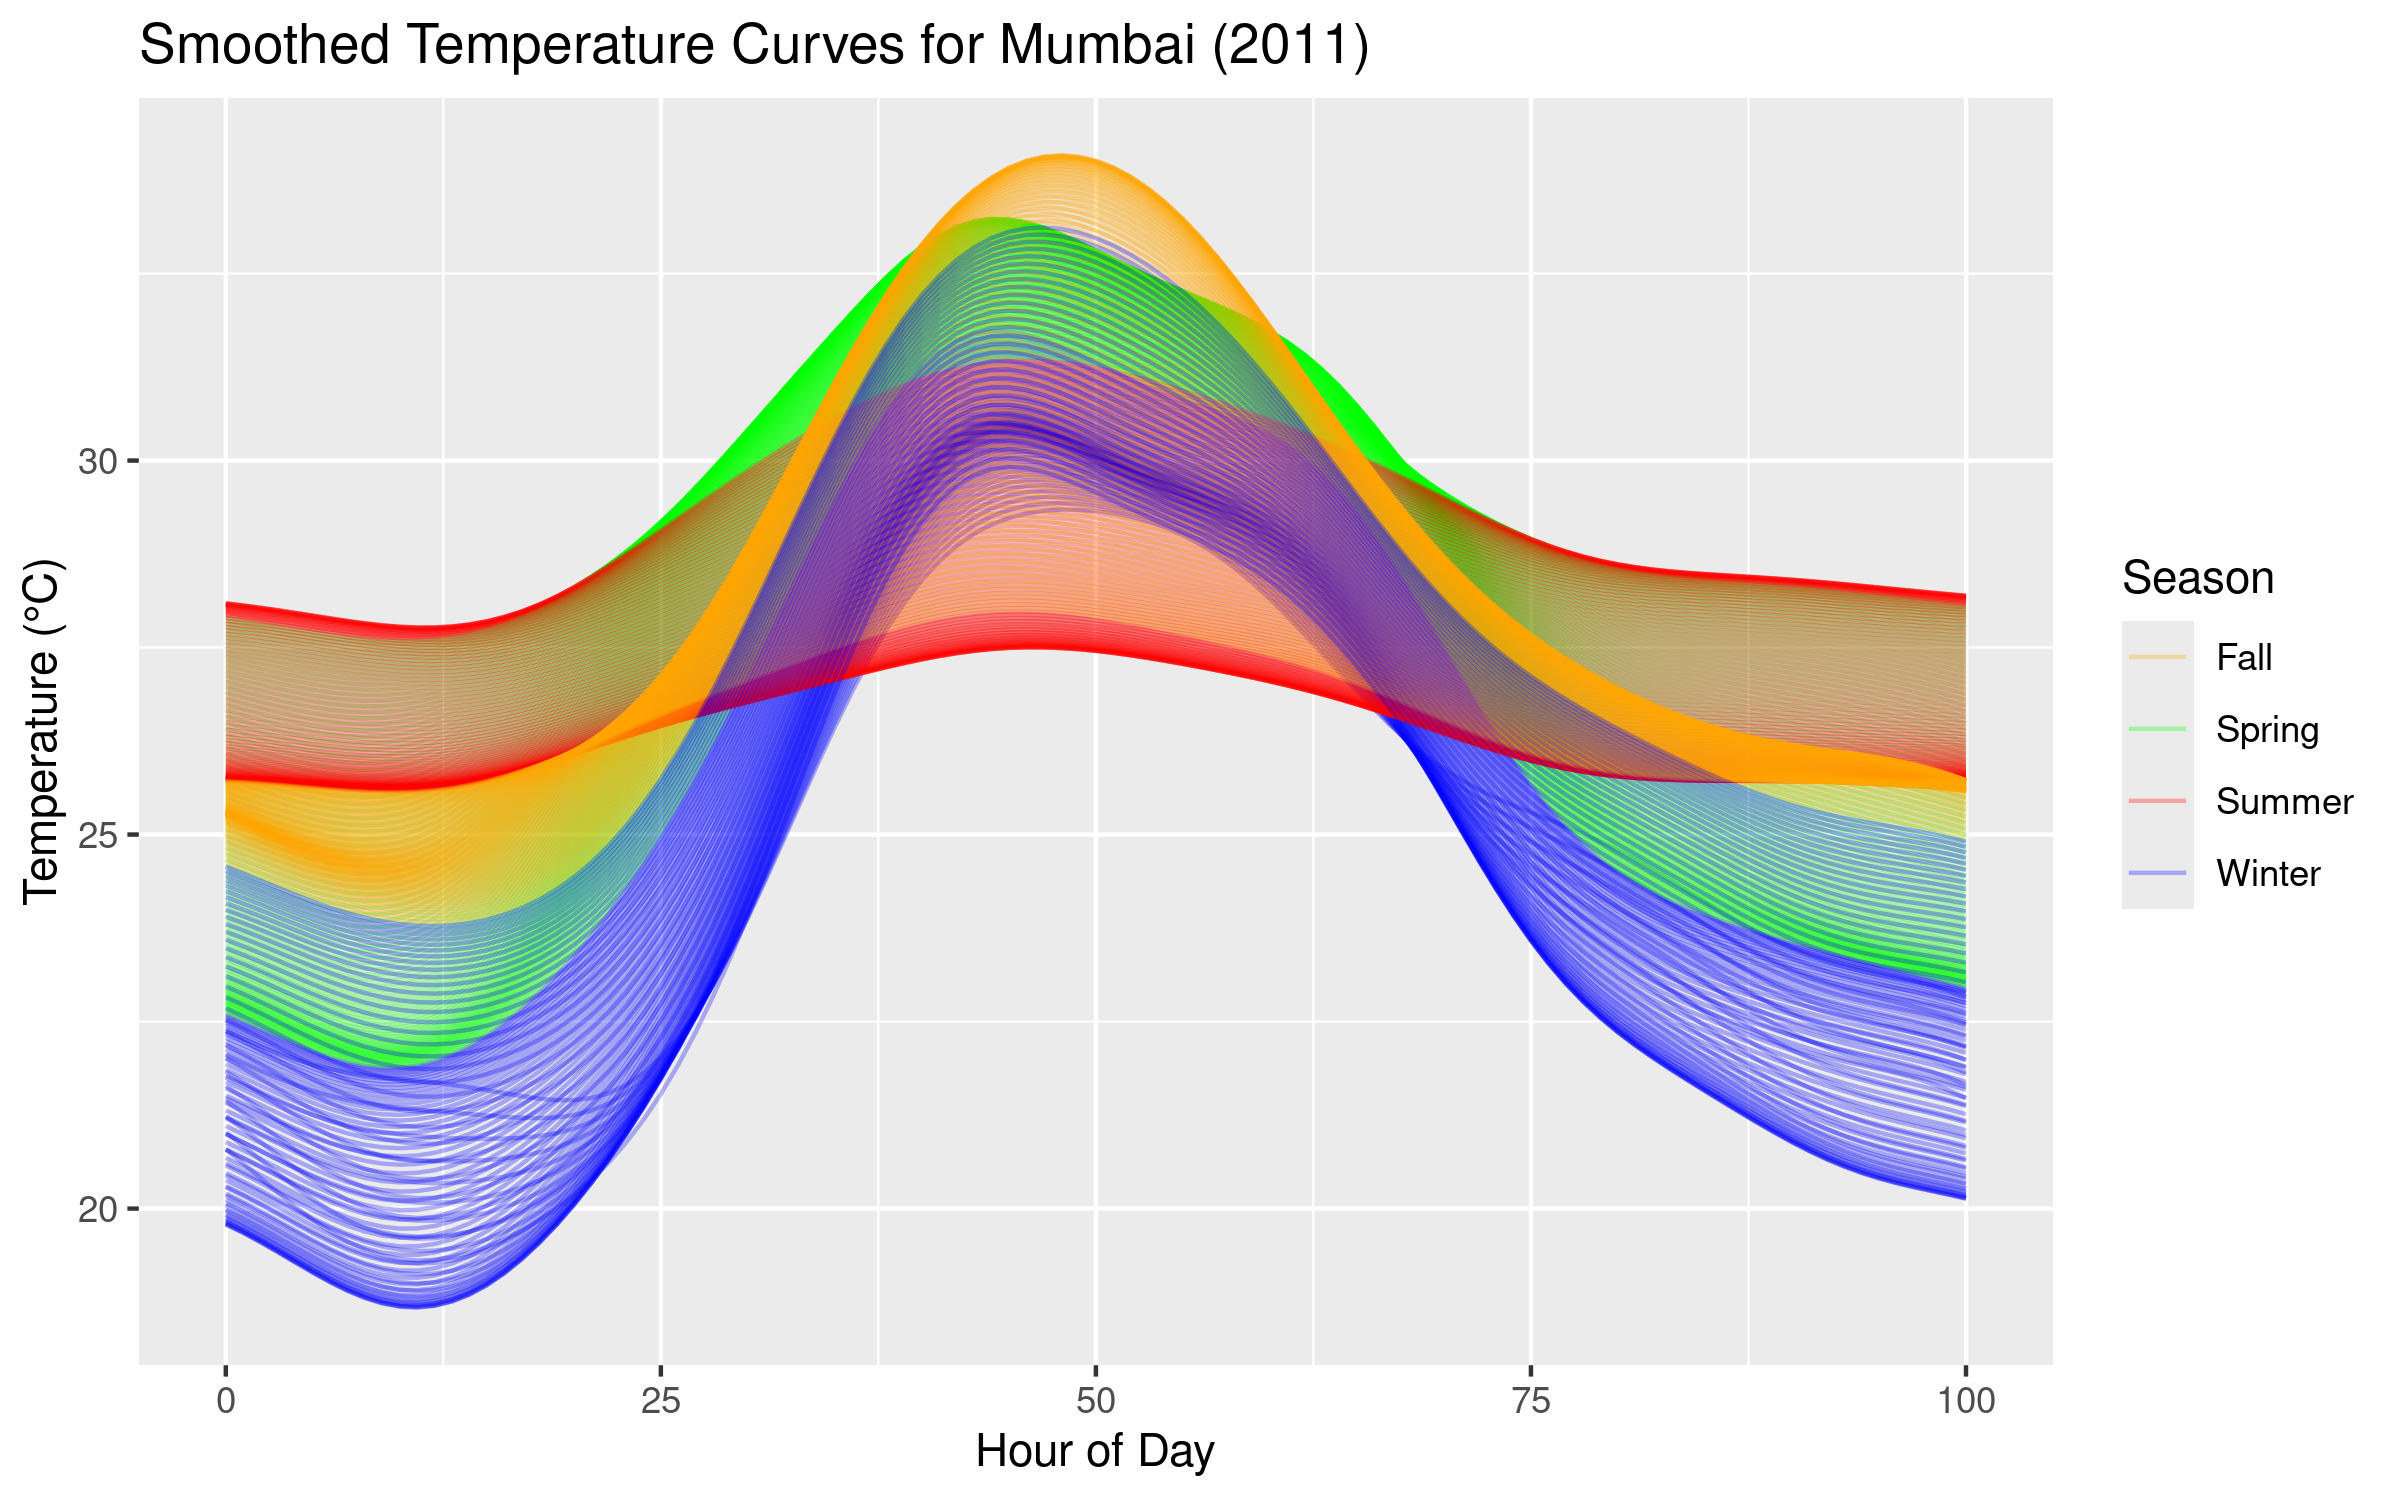
\includegraphics[width=0.8\linewidth]{../notebooks/assets/smoothed_temp_curves_mumbai.png}
	\end{center}
\end{frame}

\begin{frame}{Smoothed Temperature Curves \(Day\)}
	\begin{center}
		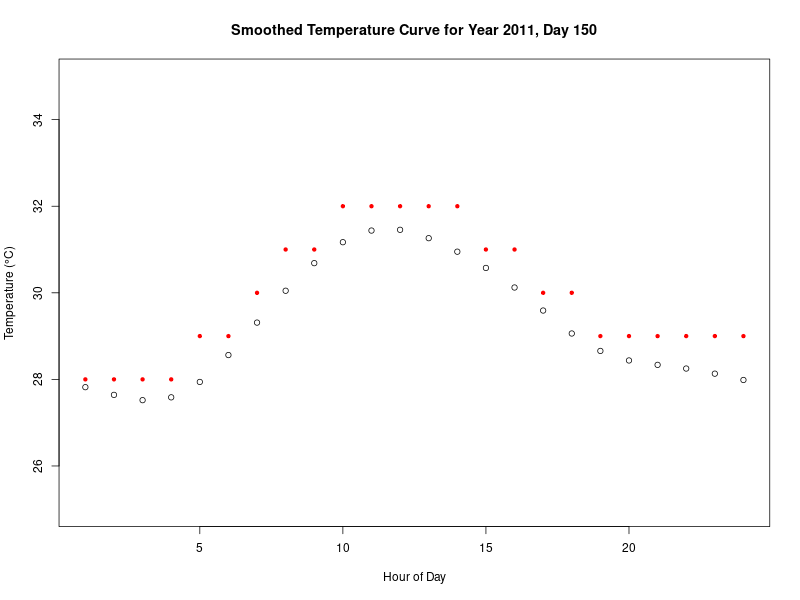
\includegraphics[width=0.8\linewidth]{../notebooks/assets/smoothed_temp_curve_day.png}
	\end{center}
\end{frame}

\begin{frame}{Smoothed Temperature Curves \(Year\)}
	\begin{center}
		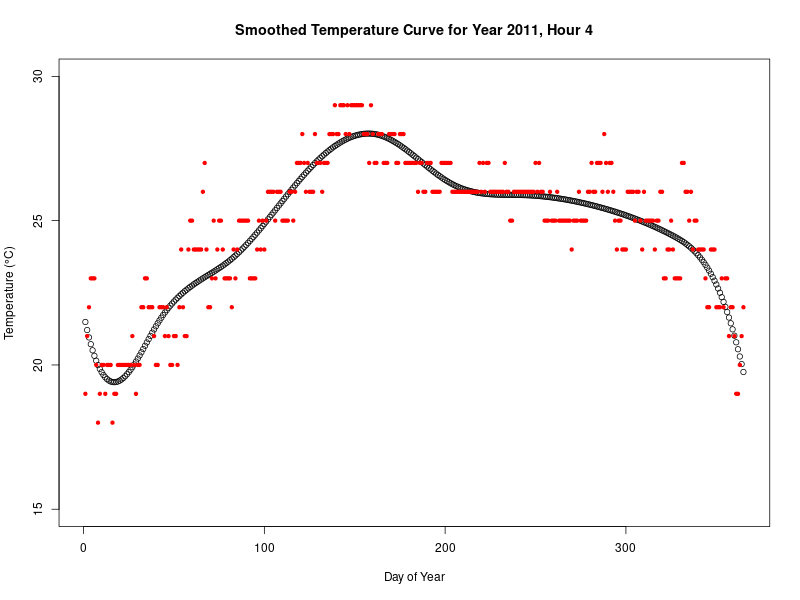
\includegraphics[width=0.8\linewidth]{../notebooks/assets/smoothed_temp_curve_year.png}
	\end{center}
\end{frame}


\section{Derivative Analysis}

\begin{frame}{First and Second Derivatives (Days)}
	\begin{itemize}
		\item First derivative: rate of change across the year
		\item Second derivative: acceleration highlights seasonal transitions
	\end{itemize}
	\begin{center}
		
\includegraphics[width=0.45\linewidth]{../notebooks/assets/derivative_day1.png}
		\hfill
		
\includegraphics[width=0.45\linewidth]{../notebooks/assets/derivative_day2.png}
	\end{center}
\end{frame}

\begin{frame}{First and Second Derivatives (Hours)}
	\begin{itemize}
		\item Intra-day temperature dynamics
		\item Captures typical morning/evening temperature dynamics
	\end{itemize}
	\begin{center}
		
\includegraphics[width=0.45\linewidth]{../notebooks/assets/derivative_hour1.png}
		\hfill
		
\includegraphics[width=0.45\linewidth]{../notebooks/assets/derivative_hour2.png}
	\end{center}
\end{frame}

\section{Covariance Structure}

\begin{frame}{Covariance Heatmap of Hourly Temperatures}
	\begin{itemize}
		\item Treat days as replicates over hours
		\item Covariance reveals which times of day co-vary
	\end{itemize}
	\begin{center}
		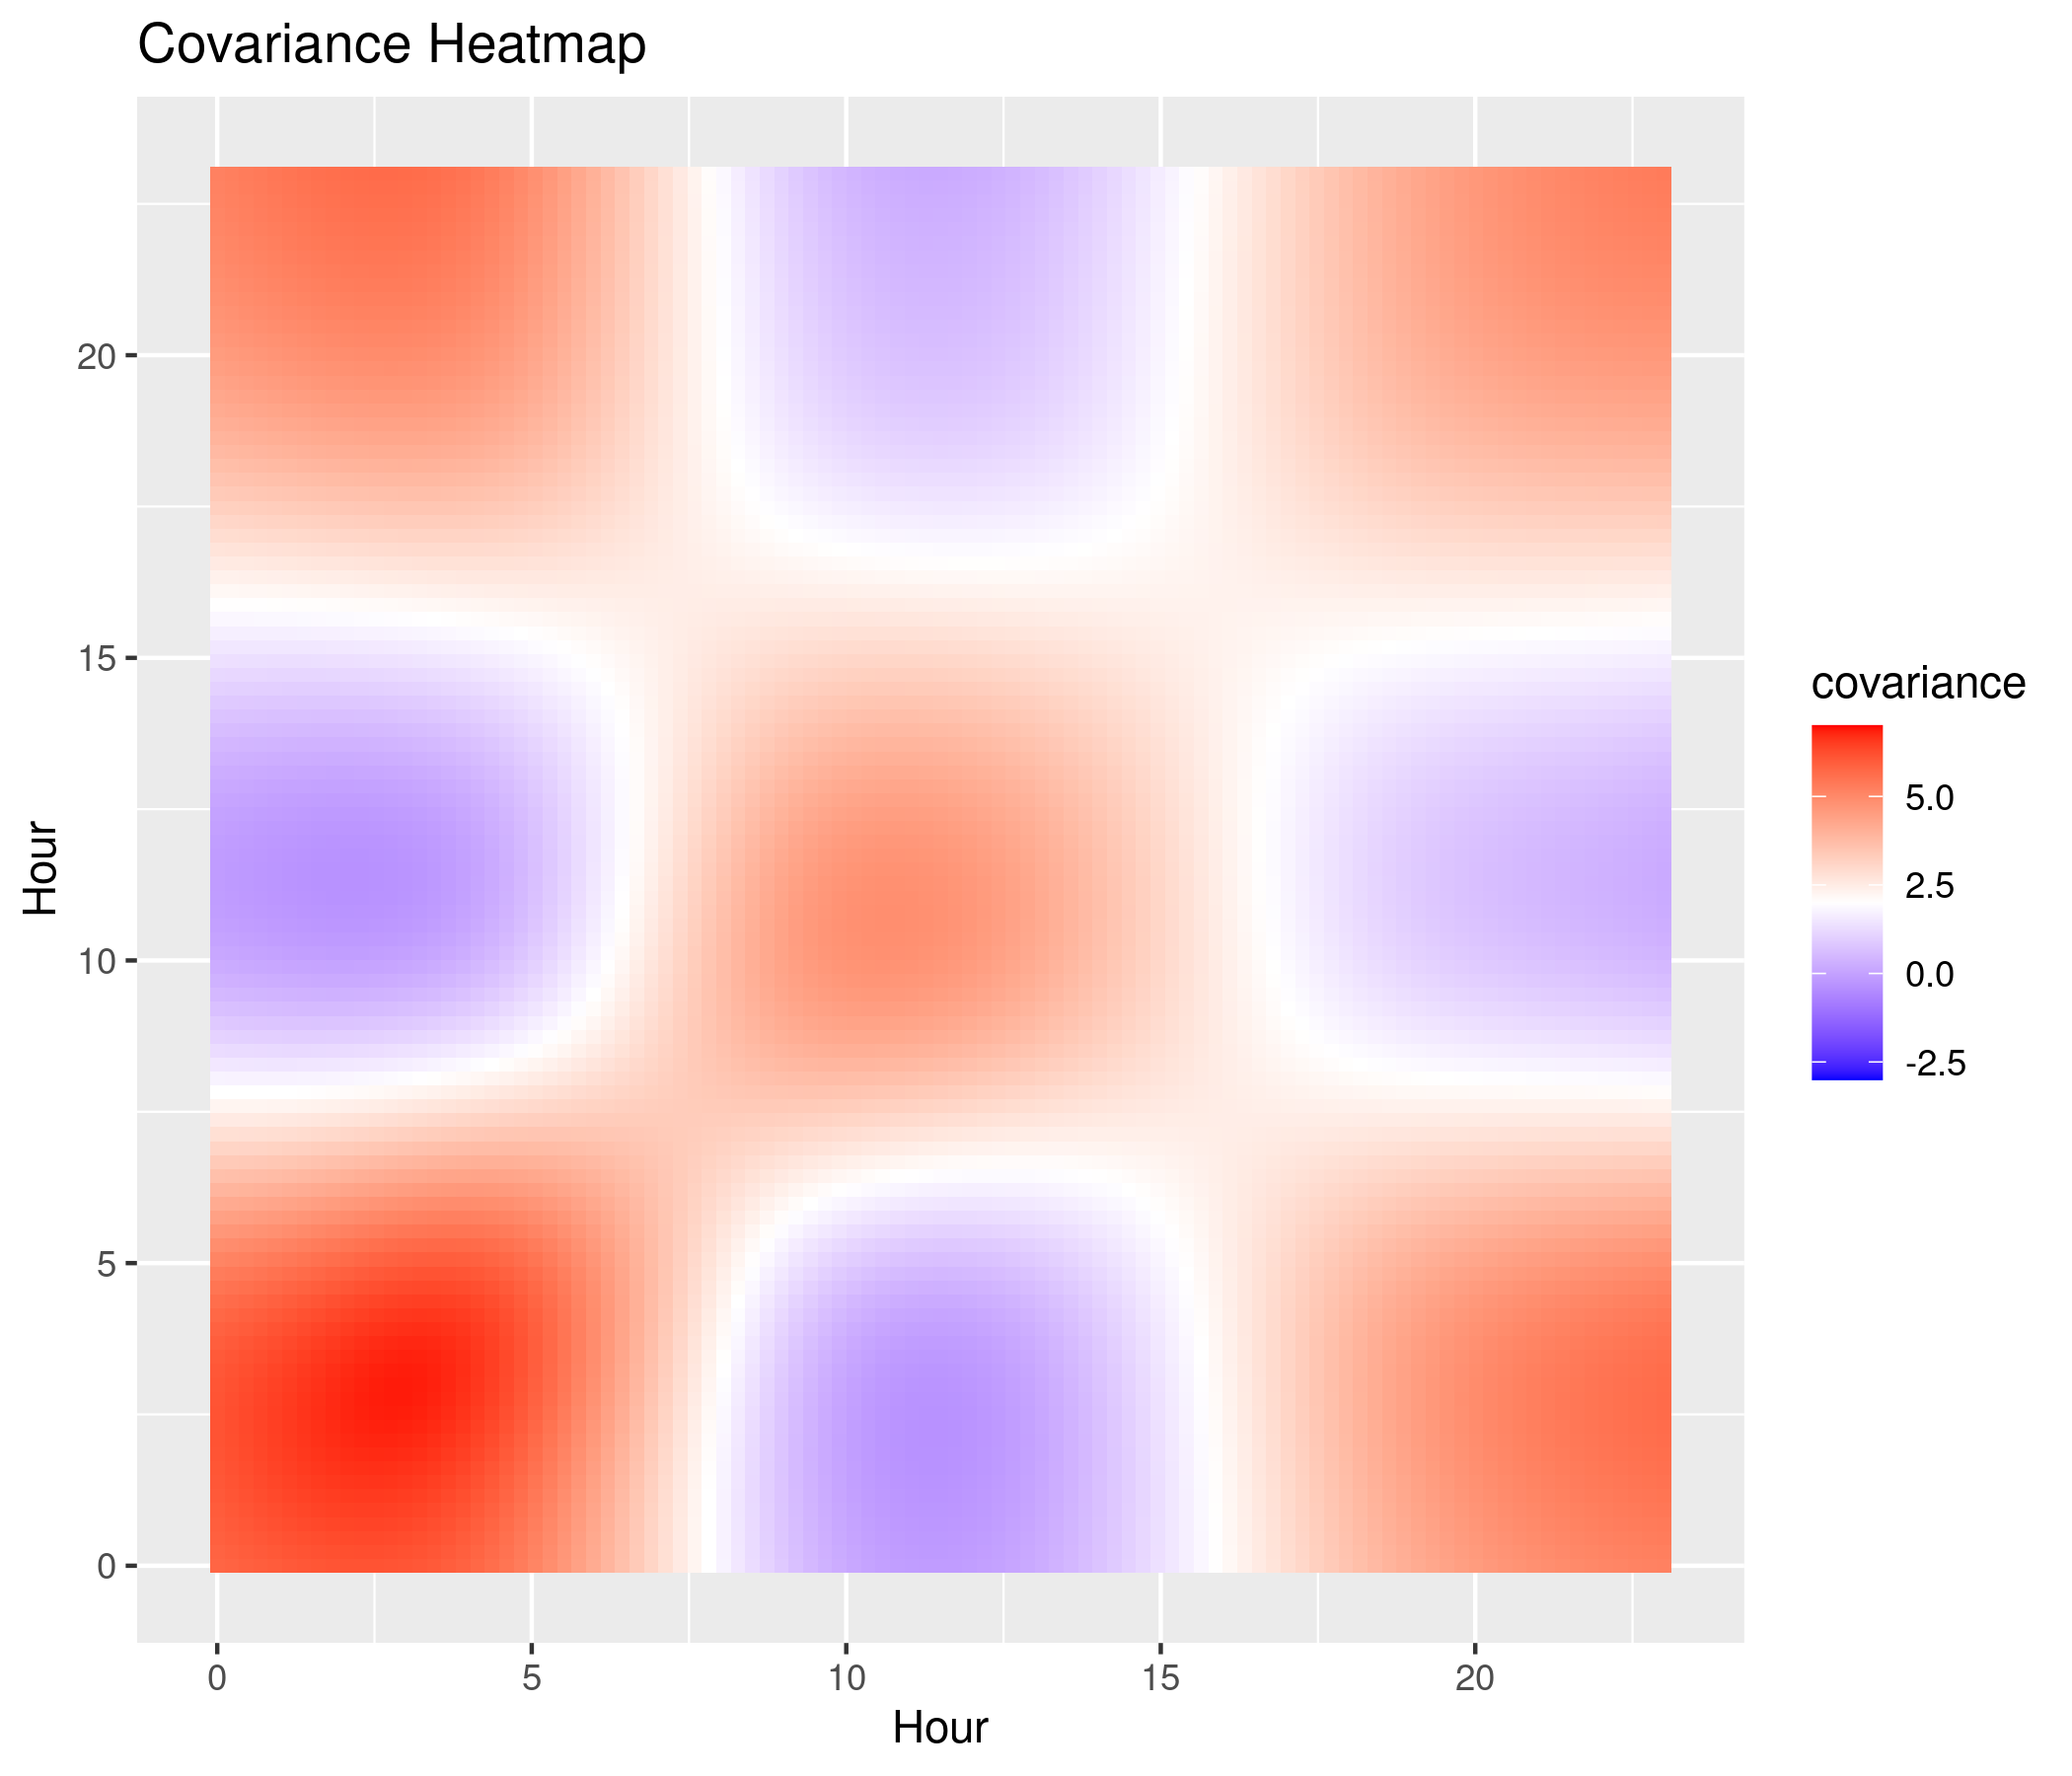
\includegraphics[width=0.68\linewidth]{../notebooks/assets/covariance_heatmap.png}
	\end{center}
\end{frame}

\section{Functional PCA}

\begin{frame}{FPCA Results}
	\begin{itemize}
		\item Principal components on smoothed bivariate functions
		\item PC1--PC3 explain over 81\% of variance
		\item Heatmaps of PC surfaces expose key modes:
	\end{itemize}
\end{frame}

\begin{frame}{First Principal Component}
	\begin{center}
		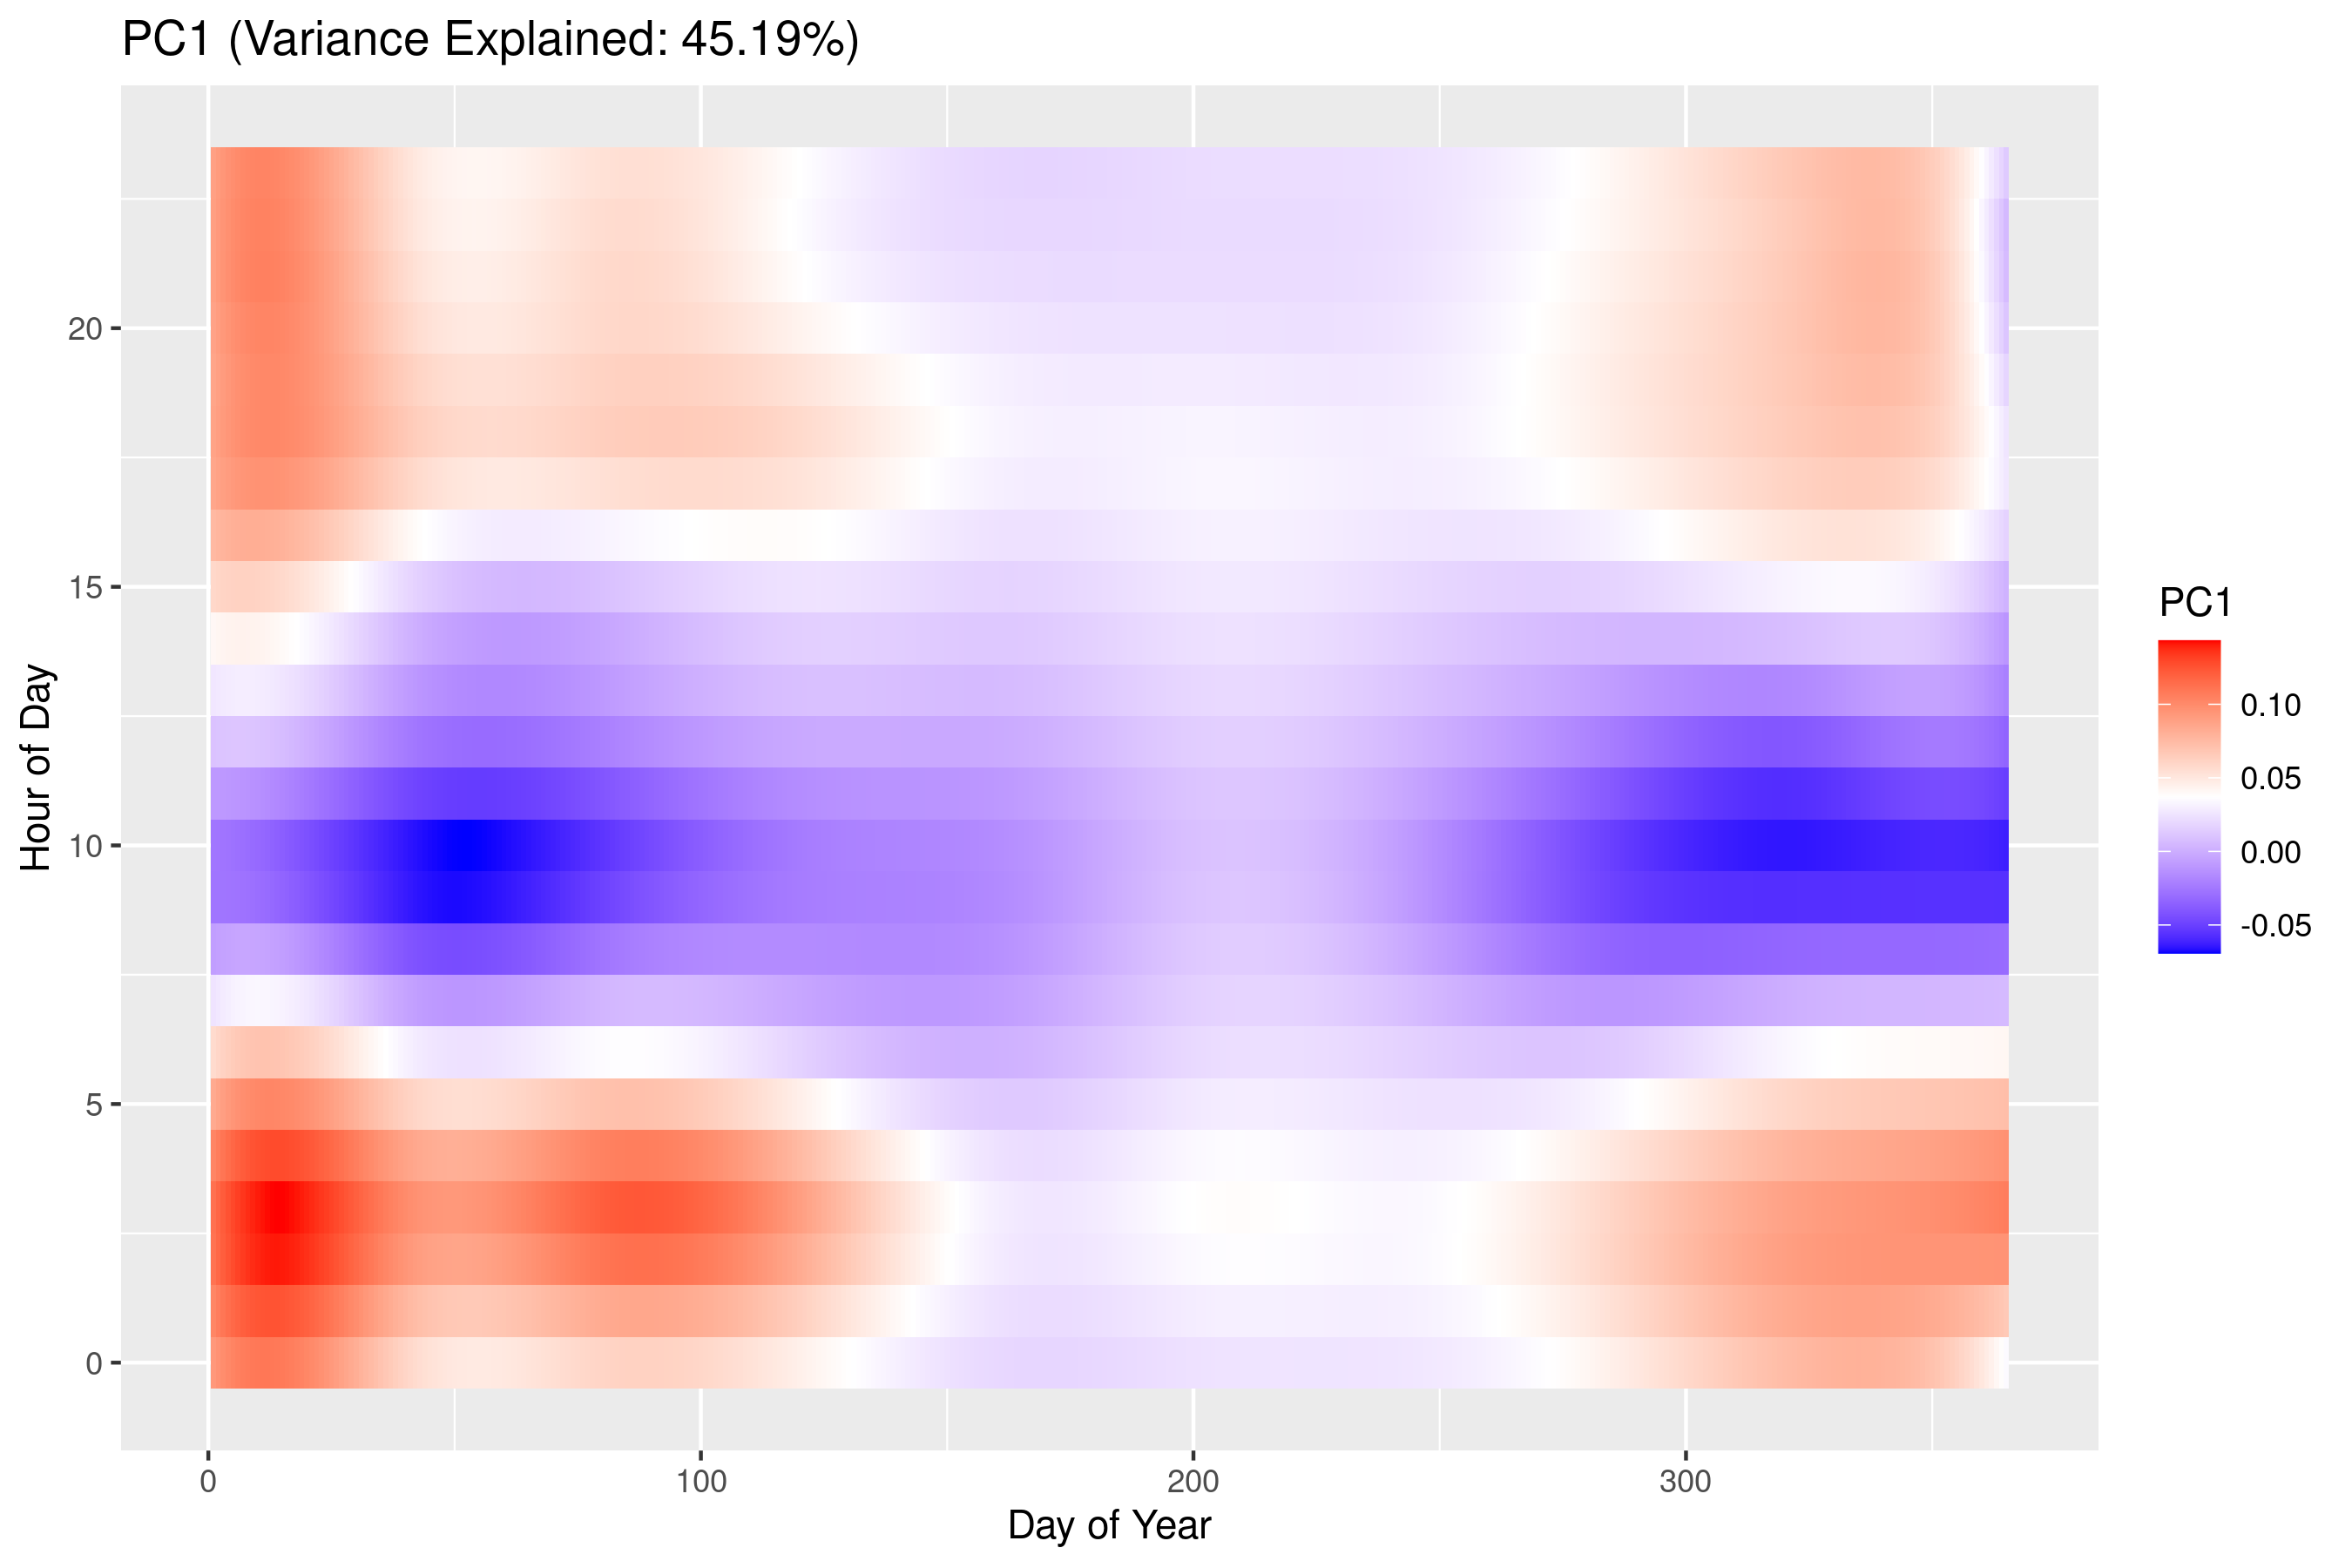
\includegraphics[width=0.8\linewidth]{../notebooks/assets/pc1_heatmap.png}
	\end{center}
\end{frame}

\begin{frame}{Second Principal Component}
	\begin{center}
		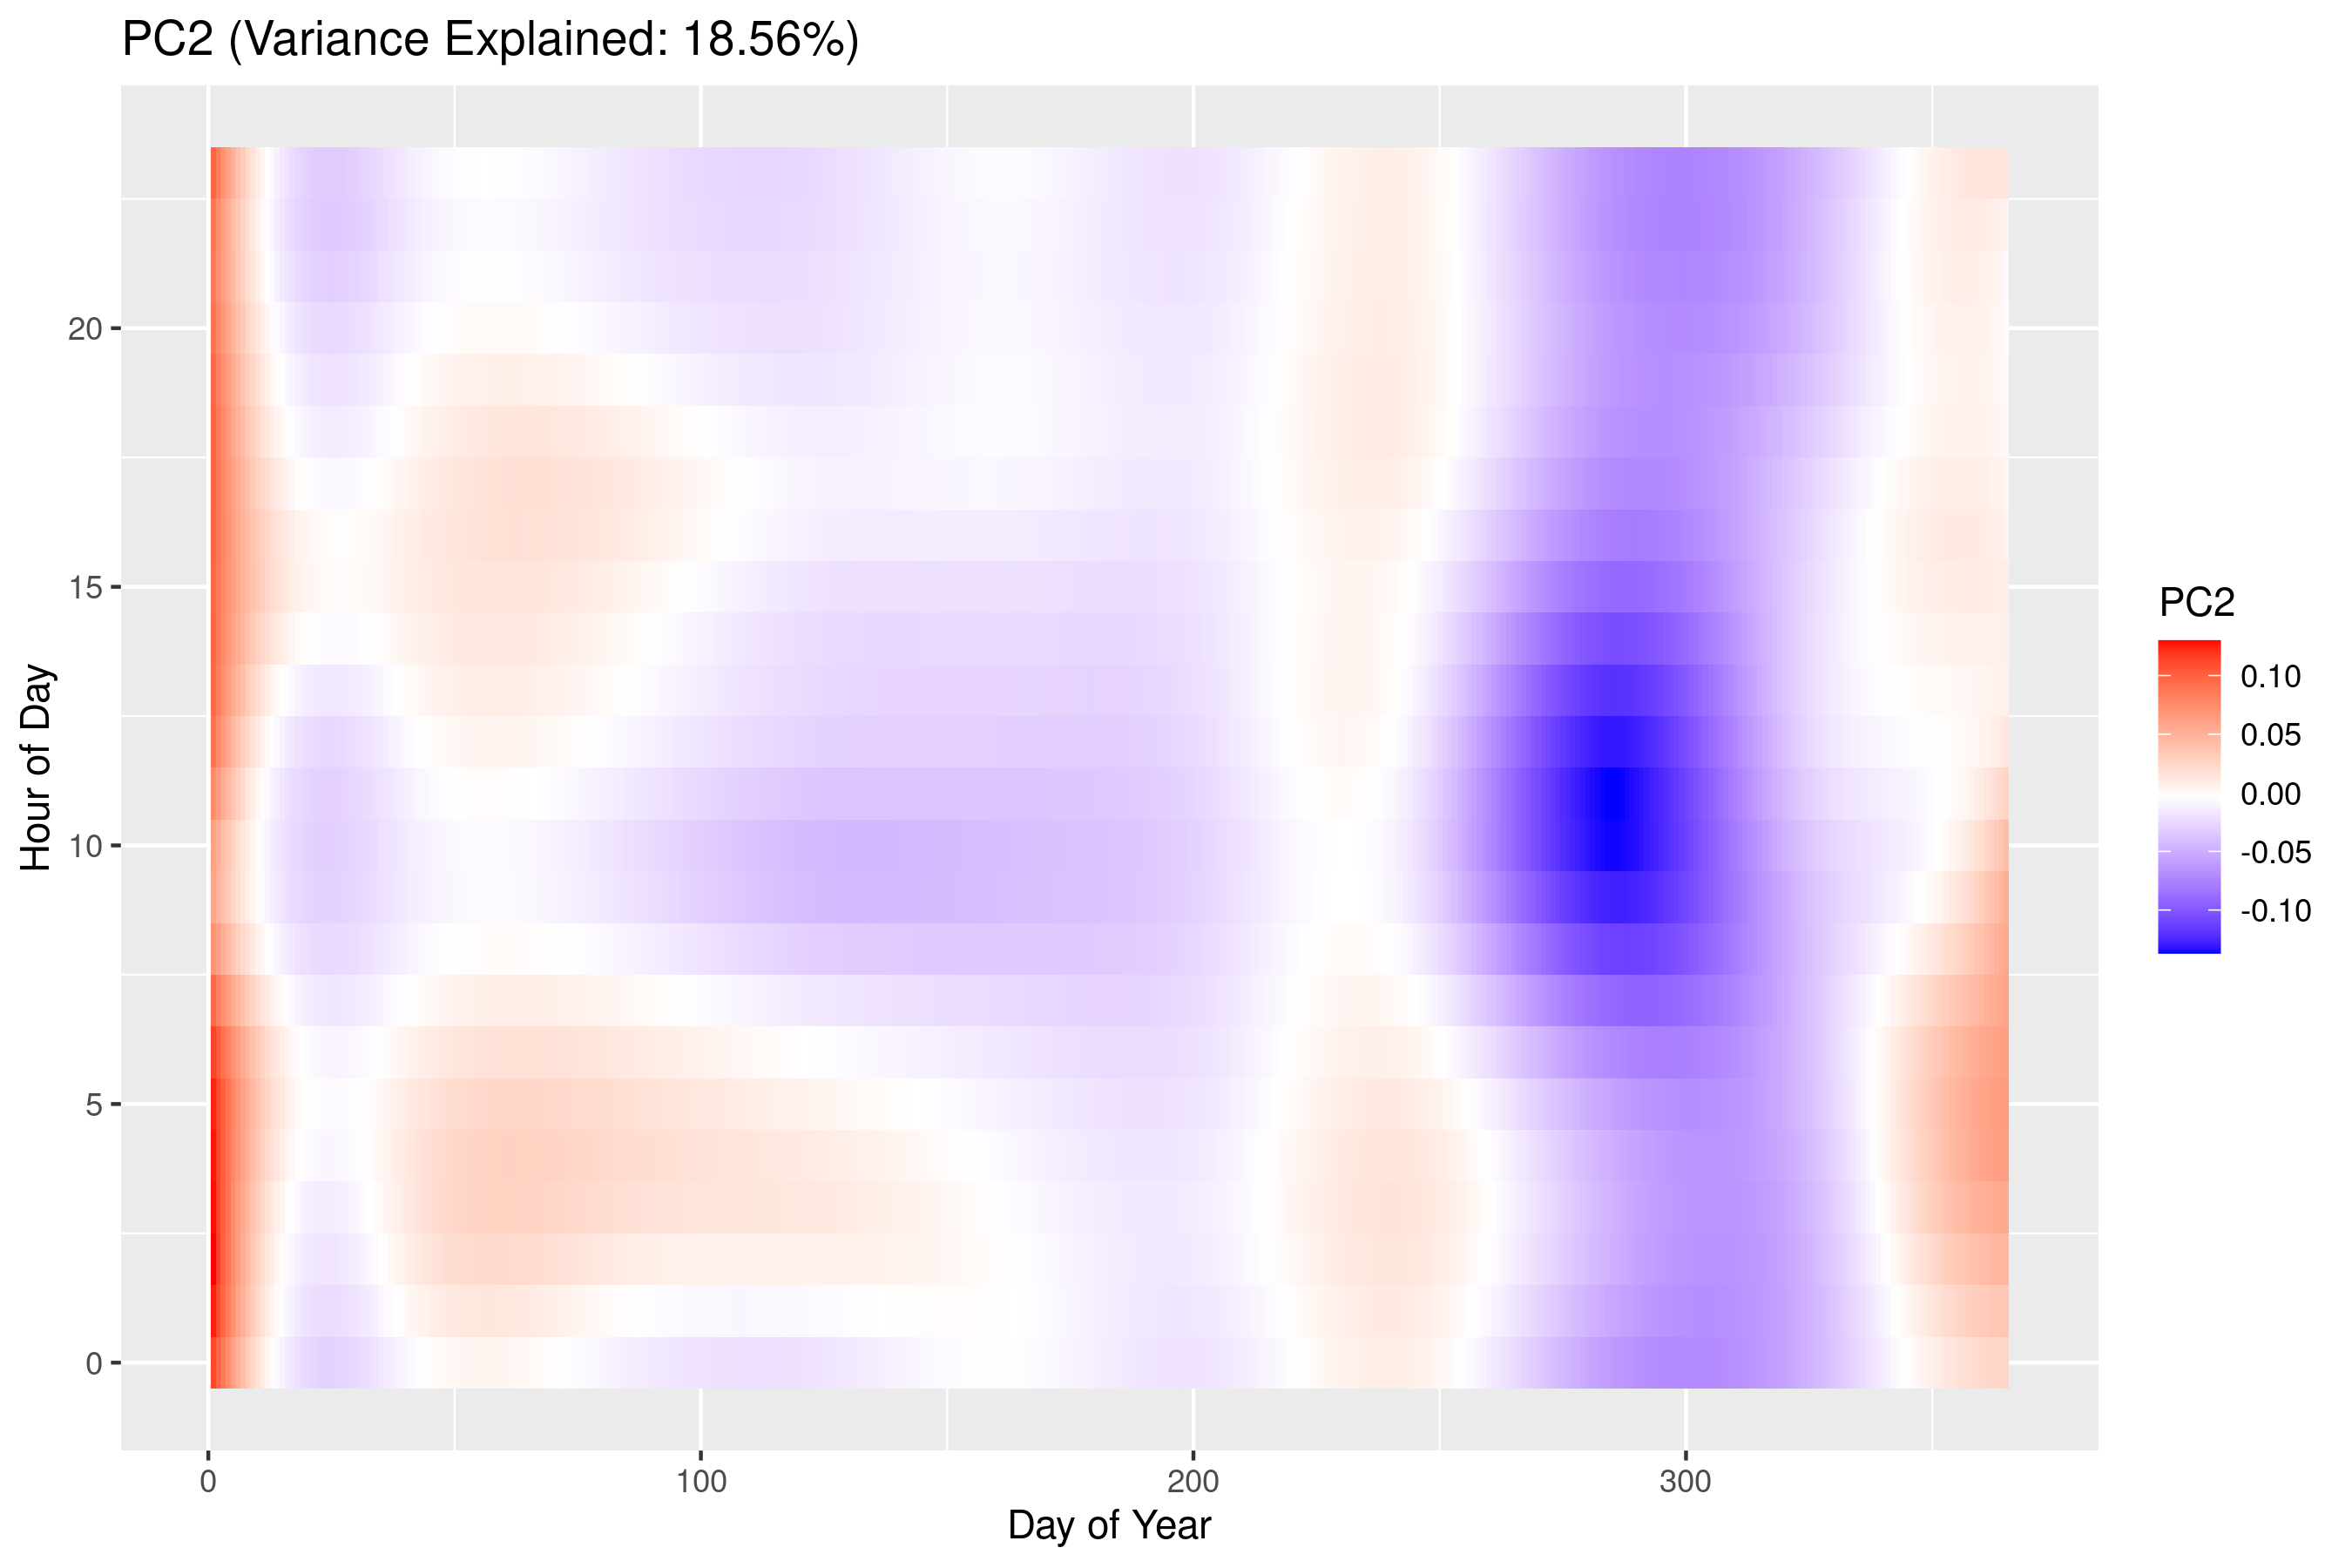
\includegraphics[width=0.8\linewidth]{../notebooks/assets/pc2_heatmap.png}
	\end{center}
\end{frame}

% \section{Curve Registration}
% \begin{frame}{Landmark Registration}
% 	\begin{itemize}
% 		\item Align daily curves by time of maximum temperature
% 		\item Reduces phase variability across days
% 	\end{itemize}
% 	\begin{center}
% 		\includegraphics[width=0.45\linewidth]{../notebooks/assets/registration_before.png}
% 		\hfill
% 		\includegraphics[width=0.45\linewidth]{../notebooks/assets/registration_after.png}
% 	\end{center}
% \end{frame}

% \section{Functional ANOVA}
% \begin{frame}{ANOVA by Season}
% 	\begin{itemize}
% 		\item Test differences in mean daily functions across seasons
% 		\item Significant seasonal effects detected (p-value < 0.01)
% 	\end{itemize}
% 	\begin{center}
% 		\includegraphics[width=0.6\linewidth]{../notebooks/assets/fanova_plot.png}
% 	\end{center}
% \end{frame}

% \section{Outlier Detection}
% \begin{frame}{Functional Boxplot and Outliers}
% 	\begin{itemize}
% 		\item Band depth used to identify outlying daily curves
% 		\item Functional boxplot displays central region and outliers
% 	\end{itemize}
% 	\begin{center}
% 		\includegraphics[width=0.7\linewidth]{../notebooks/assets/functional_boxplot.png}
% 	\end{center}
% \end{frame}

\section{Forecasting}
\begin{frame}{Annual Surface Forecast}
	\begin{itemize}
		\item FAR model on FPCA scores (VAR(1) on PC1--PC3)
		\item Forecast the next year's temperature surface
	\end{itemize}
	\begin{center}
		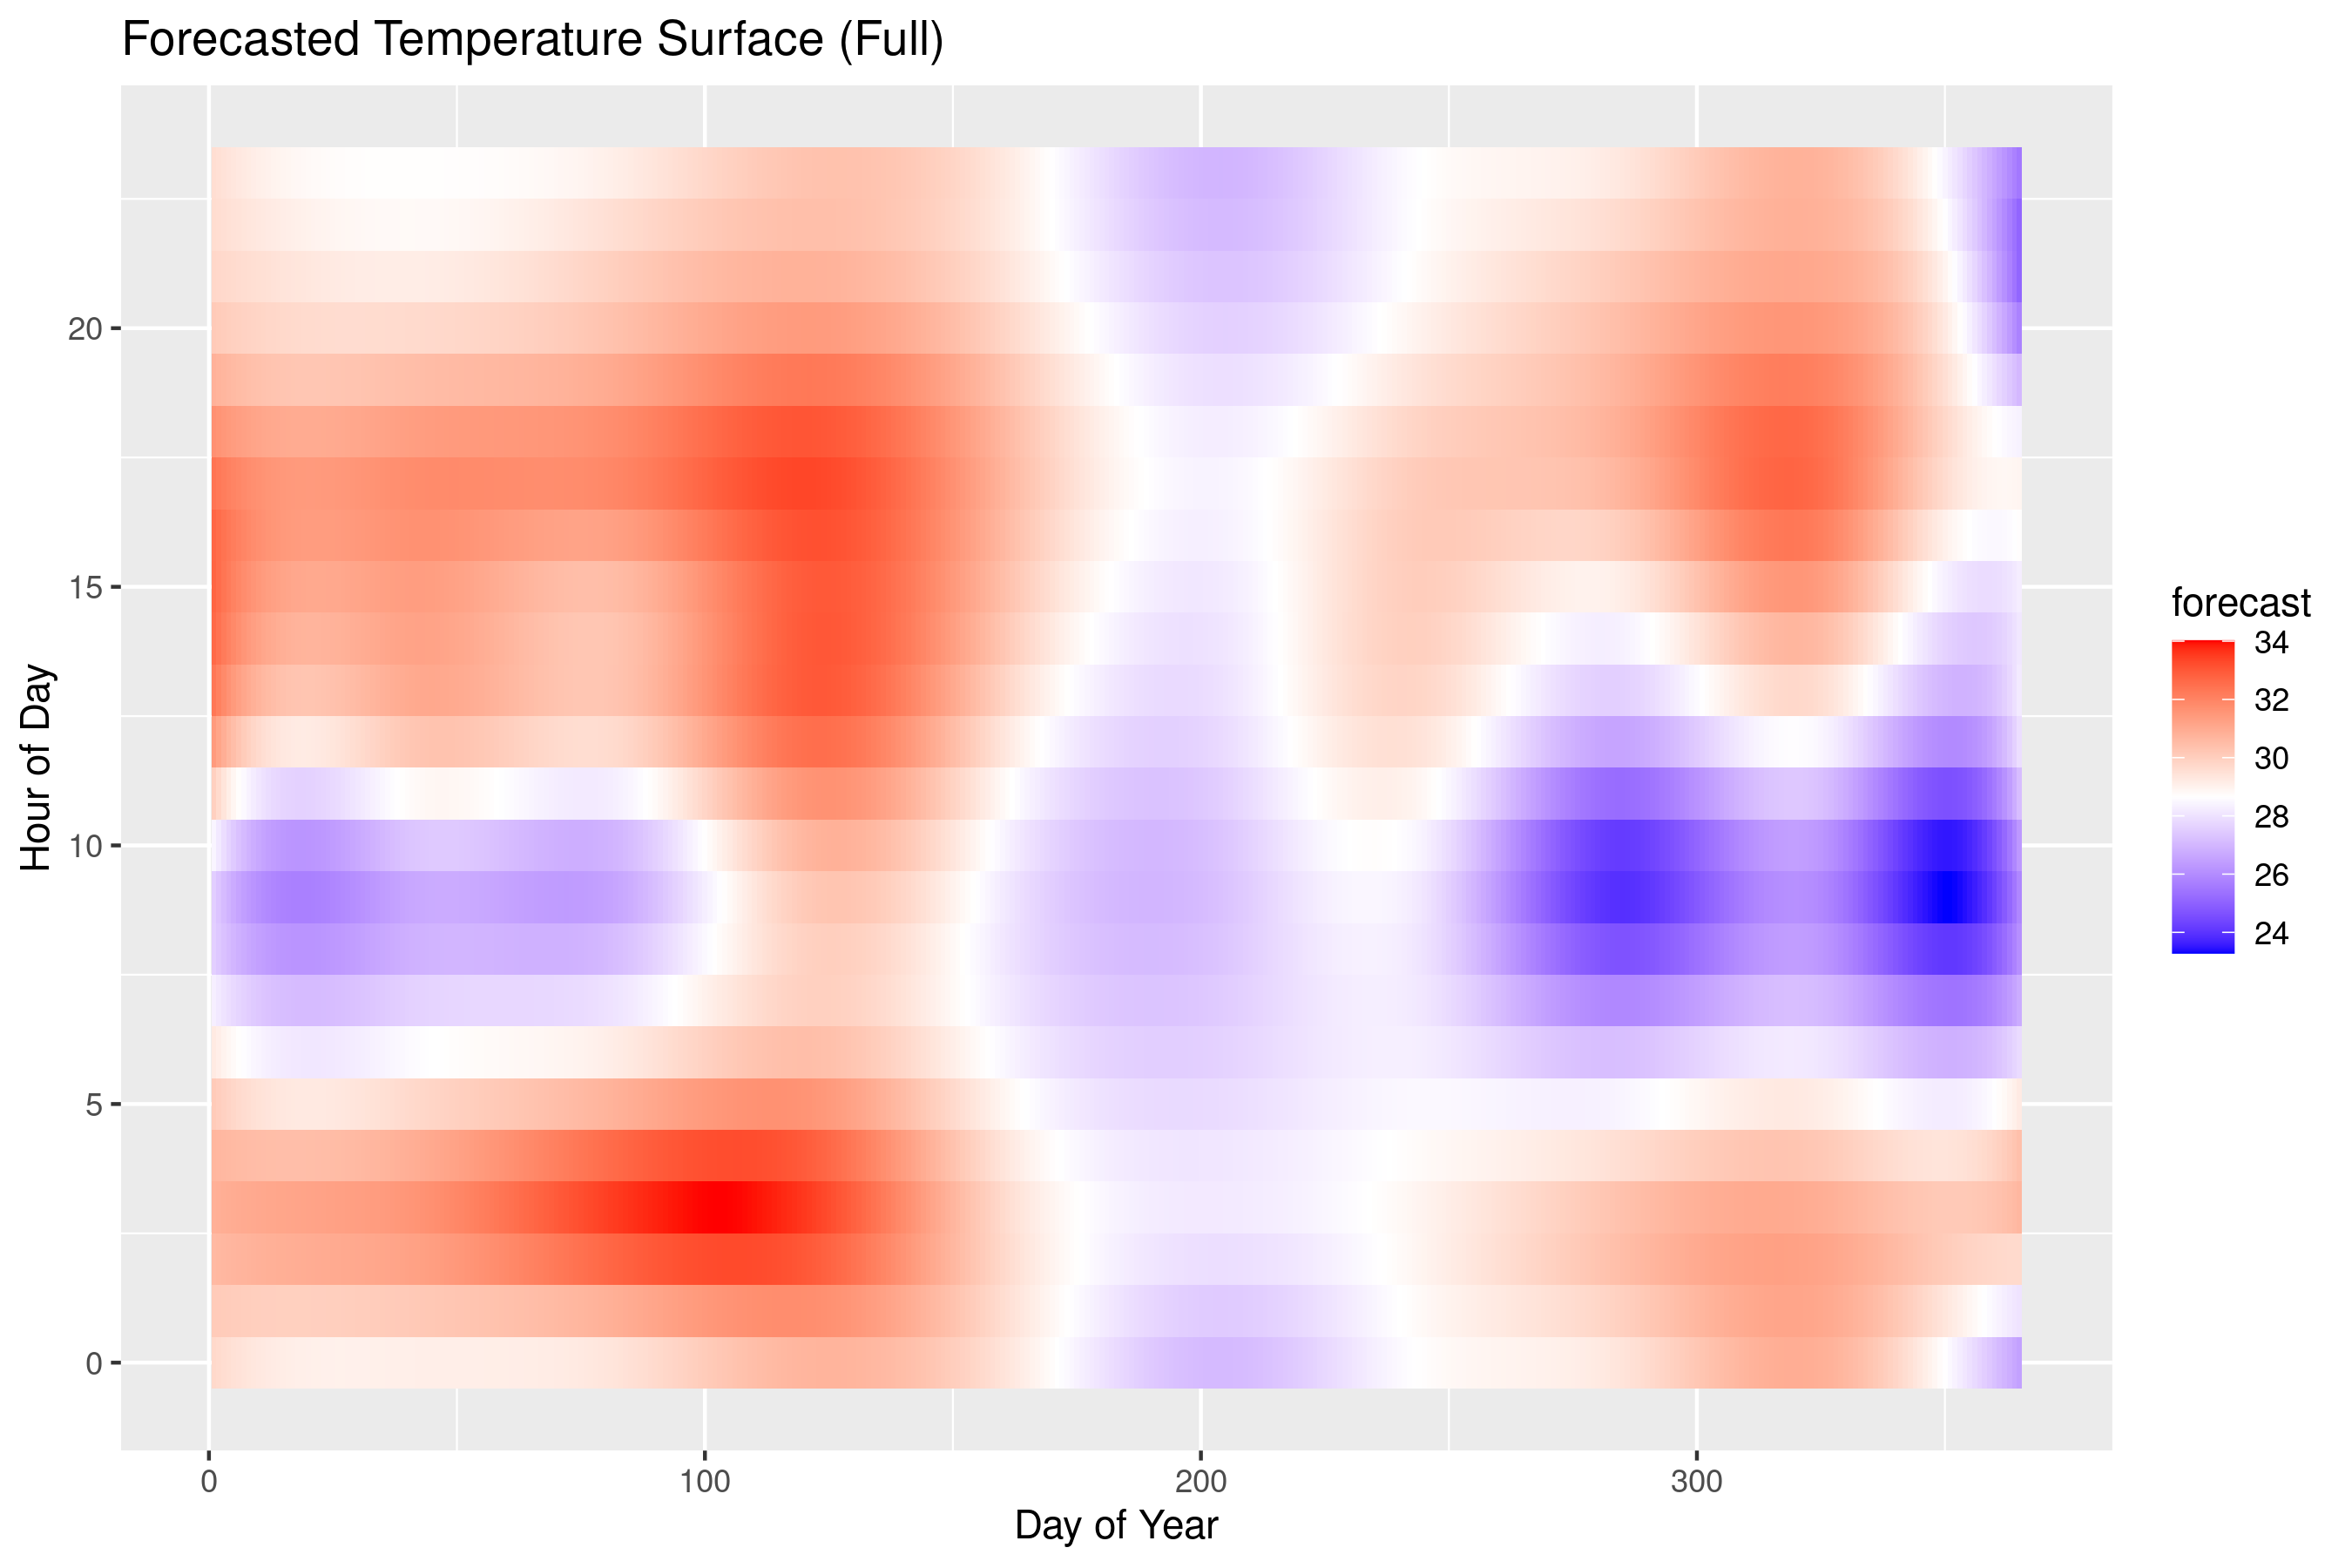
\includegraphics[width=0.7\linewidth]{../notebooks/assets/forecast_surface_full.png}
	\end{center}
\end{frame}

\section{Summary \& Next Steps}

\begin{frame}{Summary \& Next Steps}
	\begin{itemize}
		\item FDA effectively identifies seasonal patterns in weather data
		\item Even relatively 'rough' bases with capture a good part of variability
		\item Next steps:
		\begin{itemize}
			\item Hypothesis testing
		\end{itemize}
	\end{itemize}
\end{frame}

\begin{frame}{Thank You!}
	\begin{center}
		\Huge Thank you for your attention!
	\end{center}
\end{frame}

\end{document}
